\section{Background} \label{section:background}

In this section we explain the theoretical background of FPGAs and the chosen algorithm.
We also summarize the relevant related work.

\subsection{Field-programmable gate arrays}

[TODO: description of how they work]

[TODO: description of HLS]

\subsection{String matching algorithm} \label{section:background_stringmatching}

A string matching algorithm is used to find a query string, called the \textit{pattern}, within a much bigger string, called the \textit{text} \cite{makinen_compressed_2007}.
There are two kinds of string matching algorithms: sequential and indexed algorithms.
Sequential string matching relies on the original unprocessed text, which it traverses sequentially to find the requested pattern.
Indexed string matching algorithms operate on data structures constructed from the original text called an \textit{index}.
The use of specialized data structures allows for finding a pattern without searching through the whole text.
This method is preferred in the following scenarios:
Firstly, when sequentially searching the original text simply takes to much time.
Next, the text must not change often, as the whole index would have to be rebuilt.
Lastly, sufficient storage space is available to store the index.

The string matching algorithm we have chosen for our case study on the FPGA is the FM-index invented by \citeauthor{ferragina_opportunistic_2000} in \citeyear{ferragina_opportunistic_2000}\cite{ferragina_opportunistic_2000}.
The FM-index is a so-called self-index, which means that it is capable of reproducing the orignal text and its suffixes \cite{makinen_compressed_2007}.
An integral part of the efficient string matching of the FM-index is the Burrows-Wheeler transform.
Both the Burrows-Wheeler transform and the FM-index will be described in the following section.

\subsubsection{Burrows-Wheeler transform} \label{section:background_bwt}

% TODO: acronym for BWT?
The Burrows-Wheeler transformation (BWT) is an operation on a block of text $T$, which produces a permutation of the text called the Burrows-Wheeler transform $T^{bw}$, first described by \citeauthor{burrows_block-sorting_1994} in \citeyear{burrows_block-sorting_1994} \cite{burrows_block-sorting_1994}.
$\Tbw$ can often be more easily compressed than the original text and, interestingly, can be reversed to reproduce the original text.
This section will explain how the BWT works.

Creating $\Tbw$ from a block of text can be achieved using a few simple steps, as described in the original paper:

\begin{enumerate}
  \item Append a special character, here \texttt{\$}, to the original text to denote the end of the text.
  \item List all rotations of the text, by putting a character from the end of the text to the front.
  \item Sort the rotations in lexicographical ordering, where the special character \texttt{\$} has priority over any other character.
  \item $\Tbw$ is acquired by taking the last column of the matrix with the sorted rotations as rows (also known as the Burrows-Wheeler matrix).
\end{enumerate}

A graphical representation of the steps of this algorithm can be seen in figure \ref{fig:bwt} for the text \texttt{ALALA}, which will be our running example.

It may not be immediately clear how $\Tbw$ can be more easily compressed than the original text.
To better see this, take for example the string

\begin{center}
  ``\texttt{zeven\textvisiblespace schotse\textvisiblespace scheve\textvisiblespace schaatsers\textvisiblespace schaatsen\textvisiblespace scheef}''
\end{center}

which is transformed into

\begin{center}
  ``\texttt{fsenenhhaasssssvshesvshzeccccceeher\textvisiblespace\textvisiblespace\textvisiblespace\textvisiblespace\textvisiblespace tttoaaee\$}''
\end{center}

according to the ASCII character ordering.
In $\Tbw$ there are multiple runs of the same character, which can be more efficiently encoded by, for example, a run-length encoder.

To understand why these runs occur in $\Tbw$, we look at the sorted rotations in figure \ref{fig:bwt}, and especially to the last two rows.
We see that a character in the last column essentially comes before the character in the first column.
What's more, we see that there are two places in the text where an \texttt{A} precedes an \texttt{L}.
Because we sorted the rotations starting from their first character, there will be a run of the character \texttt{A} in the last column and therefore in $\Tbw$.
In most texts, there are usually only a few distinct characters that can precede a character, which results in runs in the last column \cite{burrows_block-sorting_1994}.

\begin{figure}[ht]
\centering
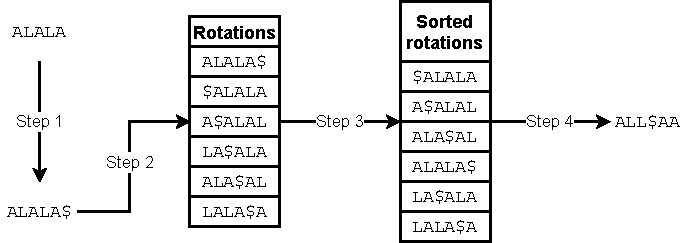
\includegraphics[width=0.8\textwidth]{figures/bwt.pdf}
\caption{The steps to acquire the Burrows-Wheeler transform of a block of text.}
\label{fig:bwt}
\end{figure}

$\Tbw$ can also be reversed to reproduce the original text.
To this end, we recognize that we can obtain the first column of the Burrows-Wheeler matrix by lexicographically sorting $\Tbw$.
Next we can use the principle of Last-First-Mapping (LF-mapping) to find a character in the first column, given the same character in the last column \cite{ferragina_opportunistic_2000}.
The LF-mapping recognizes that the ordering, or rank, of a character in the first column is the same as in the last column.
We can empirically check this by looking at the sorted rotations in figure \ref{fig:bwt}.
The first \texttt{L} encountered in the first column is the same as to the first one encountered in the last column, and vice versa for the second \texttt{L}.

The whole process of finding the original text is shown in figure \ref{fig:bwt_reverse}.
We start with the unique character \texttt{\$} which is always the last character.
Then we can find the position of \texttt{\$} in the first column using the LF-mapping.
The character preceding \texttt{\$} can then be obtained by looking in the last column on the same row.
These steps are performed until the last character is encountered again and we are done.

\begin{figure}[ht]
\centering
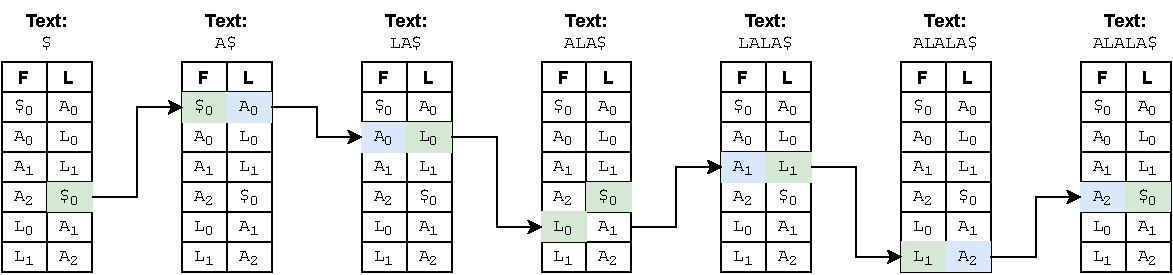
\includegraphics[width=0.99\textwidth]{figures/bwt_reverse.pdf}
\caption{Reverting the BWT to obtain the original text. F and L indicate the first and last column of the Burrows-Wheeler matrix respectively. The highlighted row in the table correspond to the LF-mapping currently being considered, and the text above the table shows the intermediate resulting text.}
\label{fig:bwt_reverse}
\end{figure}

\subsubsection{FM-index} \label{section:background_fmindex}

The FM-index is an index, which consists of the BWT and some small auxiliary array-based data structures, first described by \citeauthor{ferragina_opportunistic_2000} \cite{ferragina_opportunistic_2000}.
"FM" supposedly means "Full-text Minute-space" but could also refer to the authors \cite{langmead_introduction_nodate}.
The FM-index allows for two operations: counting the occurences of a query pattern, and finding the original position indices of the pattern in the original text.
Both operations are accompanied with an array-based data structure to speed up searching.

Finding the number of occurences of a pattern in a text also makes use the LF-mapping, just like in figure \ref{fig:bwt_reverse} where we recovered the original text from $\Tbw$.
The procedure involves keeping track of a range of rows in the Burrows-Wheeler matrix which currently match the pattern.
To demonstrate the procedure we use our running example of the text \texttt{ALALA} and the pattern \texttt{ALA}, which is shown in figure \ref{fig:bw_occurences}.
We iterate over the characters in the pattern backwards, and therefore start with matching the last character, namely \texttt{A}.
The character \texttt{A} occurs three times in the Burrows-Wheeler matrix, namely the rows starting with $A_0$, $A_1$ and $A_2$.
Using the LF-mapping property, we can then find which characters precede these \texttt{A}s.
We find that two preceding characters matching the \texttt{L} in the pattern, namely the characters $L_0$ and $L_1$.
Continuing, we further find that each of the \texttt{L}s is preceded by an \texttt{A} character, which match the first character of the pattern.
We conclude that the pattern \texttt{ALA} occurs twice in the text \texttt{ALALA}.

\begin{figure}[ht]
\centering
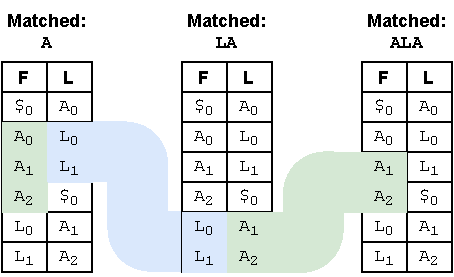
\includegraphics[width=0.5\textwidth]{figures/bw_occurences.pdf}
\caption{Iteratively finding the range of occurences of a pattern. Each table represents a Burrows-Wheeler matrix and its first and lats column. The text above the table shows the pattern that has been matched. F and L indicate the first and last column of the Burrows-Wheeler matrix respectively.}
\label{fig:bw_occurences}
\end{figure}

In practice, we do not keep track of each row that is matched.
Rather, we can save the beginning and ending row of the \textit{range} of matches.
This is possible because the Burrows-Wheeler matrix is sorted lexicographically.
Any matches are guaranteed to appear next to eachother.

Calculating the LF-mapping each time is actually very costly and therefore \citeauthor{ferragina_opportunistic_2000} propose the use of a precalculated \textit{rank matrix} \cite{ferragina_opportunistic_2000,langmead_ultrafast_2009}.
The rank matrix stores for each position in the Burrows-Wheeler matrix, how many characters have been encountered thusfar.
The rank matrix for our running example of text \texttt{ALALA} is shown in figure \ref{fig:bw_rank_matrix}.
If we start again with the rows beginning with $A_0$, $A_1$ and $A_2$ in the Burrows-Wheeler matrix, we use the rank matrix to find which \texttt{L} characters are preceding.
We see that before the range, no \texttt{L} has been encountered.
Furthermore, at the end of the range, two \texttt{L}s have been encountered.
Therefore we conclude that $L_0$ up to $L_1$ (in this case all \texttt{L}s) precede an \texttt{A}.

\begin{figure}[ht]
\centering
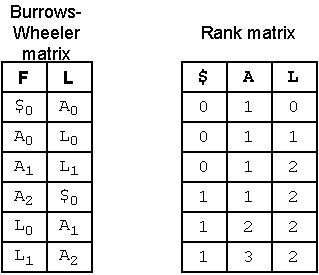
\includegraphics[width=0.5\textwidth]{figures/bw_rank_matrix.pdf}
\caption{The calculated rank matrix for a Burrows-Wheeler matrix.}
\label{fig:bw_rank_matrix}
\end{figure}

The resulting procedure \python{bw_count_occurences} is shown as pseudocode in listing \ref{listing:bw_occurences}.
The variables \python{start} and \python{end} denote the current range, and is initialized with whole range of the last character in the pattern.
Then, we loop backwards through the pattern and narrow the range to matching rows each iteration.
The auxiliary procedure \python{start_range} returns the position of the first row that start with the given character, which can be calculated in constant time due to the ordering.

\begin{listing}[ht]
% Python is easy to write pseudocode in
\begin{minted}{python}
  def bw_count_occurences(pattern):
    c = pattern[-1]
    i = len(pattern) - 1
    start, end = character_range(c)
    while start <= end and i > 0:
      c = pattern[i-1]
      start = start_range(c) + count_occurences(c, start-1)
      end = start_range(c) + count_occurences(c, end-1)
      i -= 1

    if end < start:
      return 0
    else
      return end - start
\end{minted}
\caption{Pseudocode for finding the number of matches of a pattern in a text.}
\label{listing:bw_occurences}
\end{listing}

Having found the range of starting characters for our pattern, we want to find their positions in the original text as well.
To this end, we can use an additional data structure, called the suffix array \cite{langmead_burrows-wheeler_1994}.
A suffix array stores for each character in $\Tbw$ the position in the original text that the character corresponds to.

In figure \ref{fig:bw_suffix_array}, the suffix array is shown for our running example of the text \texttt{ALALA}.
We are finally ready to identify where the pattern \texttt{ALA} occurs in the original text.
We have previously found that the \texttt{A}s with rank one and two are the starting positions of the pattern within the text.
These in turn correspond to the last two \texttt{A}s in $\Tbw$.
Consulting the suffix array in figure \ref{fig:bw_suffix_array} tells us the pattern occurs at index zero and two in the original string.
It can be easily checked that this is correct.

\begin{figure}[ht]
\centering
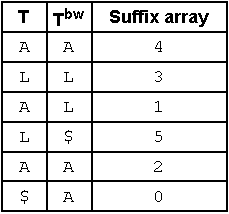
\includegraphics[width=0.35\textwidth]{figures/bw_suffix_array.pdf}
\caption{The original text $T$ (\texttt{ALALA}), its Burrows-Wheeler transform $\Tbw$ and the suffix array are shown alongside eachother.}
\label{fig:bw_suffix_array}
\end{figure}

\section{Related Work} \label{section:related_work}

In this section, we summarize two case studies on performance of high-level models (OpenCL in particular).

\subsection*{Optimizing OpenCL Code for Performance on FPGA: k-Means Case Study With Integer Data Sets \cite{zohouri_evaluating_2016}}

In this work the authors present three programming techniques to optimize OpenCL HLS performance.
Using these techniques, they further show that FPGAs can outperform CPUs for certain algorithms.
The first technique they show is explicit vectorization of loops in the algorithm.
This replaces a loop with operations that can be parallelized.
Secondly, the authors show an NDRange approach where a task is split into independent parts that are executed by separate kernel.
Finally, they show that data transfer between the host system and the kernels can sometimes be done in bursts depending on the amount of memory on-board, to limit the number of transfers while transferring as much data as possible at once.
However, the data-transfer technique could result in non-portable code.

The paper shows how these optimizations lead to 1.5x speedup for four of twelf experiments conducted.
Moreover, no matter what optimization applied, using the FPGA to offload the algorithm results in 60\% to 80\% less energy consumption.

\subsection*{Evaluating and Optimizing OpenCL Kernels for High Performance Computing with FPGAs \cite{paulino_optimizing_2020}}

This paper presents several programming techniques to improve the efficiency of running OpenCL benchmarks on FPGAs.
Firstly, using OpenCL annotations, one can indicate that a kernel can be replicated as separate pipelines to exploit data parallelism.
Other optimizations are loop unrolling and using a shift register when performing calculations on floating-point numbers.
Finally, for algorithms that exhibit a structured grid computation pattern, the advanced sliding window technique can be used.
The authors investigate the performance benefits of these techniques using benchmarks from the Rodinia suite.
Experimental results from these benchmarks show that FPGAs are slightly faster than CPUs, but not better than GPUs.
The FPGAs are however up to 3.4x more energy efficient than GPUs at executing the benchmarks.

[TODO: also include paper about FM-index acceleration on FPGAs]
